%
% File main.tex
%
% Contact: car@ir.hit.edu.cn, gdzhou@suda.edu.cn
%%e.agirre@ehu.es or Sergi.Balari@uab.es
%% and that of ACL 08 by Joakim Nivre and Noah Smith

\documentclass[11pt]{article}
\usepackage{acl2015}
\usepackage{times}
\usepackage{url}
\usepackage{latexsym}
\usepackage{graphicx}



\makeatletter
\newcommand{\@BIBLABEL}{\@emptybiblabel}
\newcommand{\@emptybiblabel}[1]{}
\makeatother
\usepackage{hyperref}

%\setlength\titlebox{5cm}

% You can expand the title box if you need extra space
% to show all the authors. Please do not make the title box
% smaller than 5cm (the original size); we will check this
% in the camera-ready version and ask you to change it back.


\title{Spoiler detection and extraction\\POC for NLP Course, Winter 2022}

\author{M. Kierznowski, Ł. Pancer, P. Wesołowski \\
  Warsaw University of Technology \\
%   {\tt email@domain} \\
  \And
    supervisor: Anna Wróblewska \\
  Warsaw University of Technology \\
    {\tt anna.wroblewska1@pw.edu.pl}
    }

\date{}

\begin{document}
\maketitle
\begin{abstract}
This document presents exploratory data analysis, describes current experiments, and provides preliminary results for the first NLP course project. The project addresses the spoiler detection task. The main goal is to evaluate the performance of the spoiler classification models through an interpretability-based technique, i.e., compare their critical phrases with the ones annotated. So far, we have focused on creating machine-learning models. The next step will be to use XAI tools on them.

\end{abstract}

\section{Introduction}
As an introduction, let us remind that we aim to analyze models dealing with the classification of entire reviews as containing a spoiler or not. Once the relevant models have been created, we will attempt to compare the sets of words that influence the decision to classify as a spoiler and annotated segments. Moreover, we hope to identify other interesting properties of the models.

We have focused on three datasets, namely:
\begin{itemize}
    \item Goodreads - 1.3M documents, 17M sentences, 570k spoiler sentences \cite{wan2019fine},
    \item TV Tropes Books - 340k documents, 670k sentences, 110k spoiler sentences \cite{wroblewska2021spoiler},
    \item IMDB reviews - 5.5M documents, 1.1M spoiler \cite{enam_biswas_2021}
\end{itemize}
Their properties are further examined in section~\ref{eda}.

\section{Exploratory data analysis} \label{eda}


\subsection{Goodreads}

This data set may be found in two forms: balanced, which is used in provided research, and standard. We have selected the balanced alternative in order to provide research on at least one balanced dataset.
Moreover, it contains sentence-level annotation, indicating which sentences carry unwanted information. For these sentences (assigned to accommodate spoilers), the frequency distribution of words is provided in figure \ref{fig:freq-dist}. Note that before calculations, stop words were deleted (downloaded from the nltk package) as well as punctuation marks such as "," or ".".

\begin{figure}[h]
    \centering
    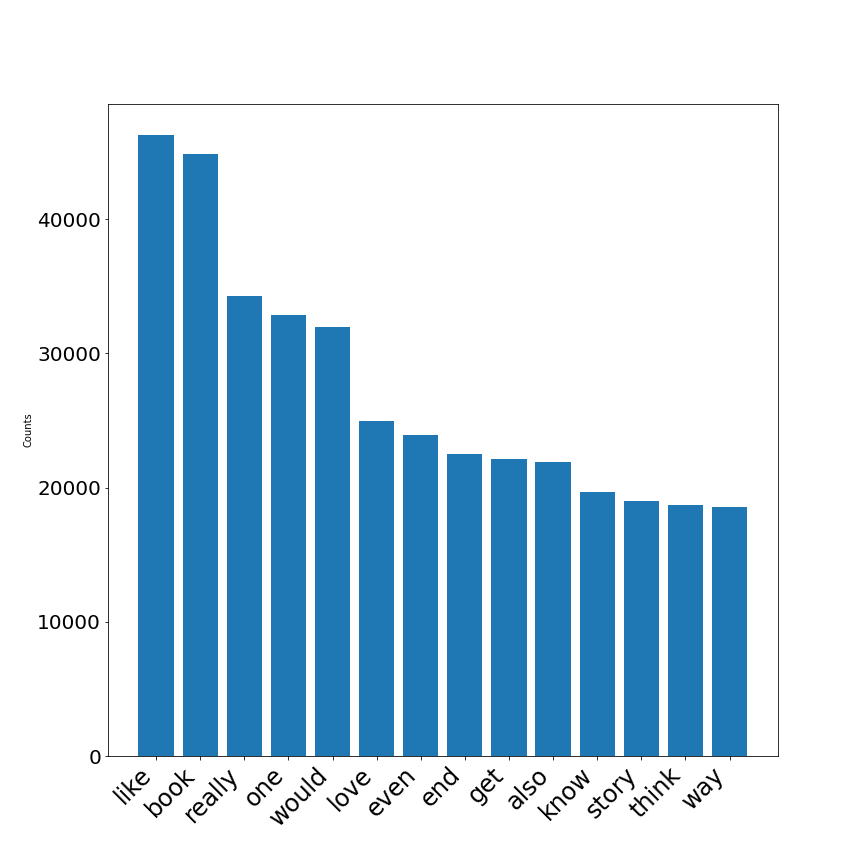
\includegraphics[width=\columnwidth]{img/FreqDistFiqure.png}
    \caption{Frequency Distribution of sentences containing spoiler for Goodreads dataset} 
    \label{fig:freq-dist}
\end{figure}

Analyzing provided figure, we can presume that words such as \emph{love}, \emph{know}, or \emph{story} may hold undesirable content.

Finally, one important issue is worth elaborating on. We focus on the whole review classification. Moreover, our models are BERT-based, which means they can handle up to 512 input tokens. The reviews where the first spoiler occurs after the first 512 tokens may be problematic. We investigated this topic further and estimated that about 90\% of spoiler reviews contain at least one spoiler within the first 512 tokens. Therefore, we decided to leave it as it is. Besides, who knows if the model cannot learn if the review contains spoilers on the basis of only part of it? (but, e.g., the author's writing style, etc.).

\subsection{TV Tropes Books}

This dataset provides more detailed information about spoilers. It also contains word-based information. However, it also lays out which specific words are spoilers.

Applying frequency distribution of words among spoilers sentences provides compelling information about specific words, as shown in figure~\ref{fig:freq-dist-troop}.

\begin{figure}
    \centering
    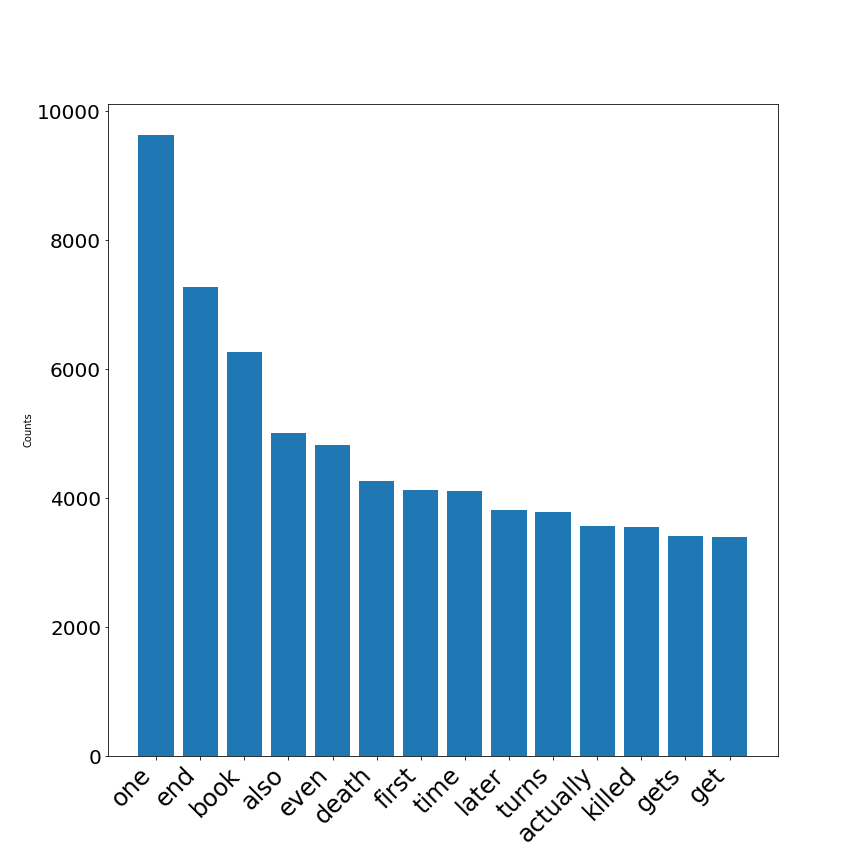
\includegraphics[width=\columnwidth]{img/FreqDistFiqure_Troops.png}
    \caption{Frequency Distribution of sentences containing spoiler for TV Tropes Books dataset} 
    \label{fig:freq-dist-troop}
\end{figure}

Figure \ref{fig:freq-dist-troop} reveals words that may strongly contribute to spoilers, such as \emph{death} or \emph{killed}. Looking closer at those trigger words may contribute to finding some specific pattern. 

\subsection{IMDB reviews}
Contrary to the other two datasets, the IMDB reviews set contains only document-level annotations. Therefore, we cannot extract as much information from this dataset as in previous cases.

Two sample records from this dataset are shown in table \ref{tab:imdb-sample}.

The dataset is highly imbalanced, as shown in figure \ref{fig:imdb-classes}. It features roughly 1.2M non-spoiler reviews and 4.4M spoiler-tagged reviews.

Regarding review lengths, there are 32 outliers containing more than 200 sentences. There are 625 reviews which consist of more than 100 sentences. Figure \ref{fig:imdb-sentence-hist} shows a histogram of review length in terms of the number of sentences. Note that reviews featuring more than 100 sentences are not included. One can see that the vast majority of sentences are shorter ones, with less than 20 sentences.

Due to the very high volume of this dataset, we decided to remove randomly excessive reviews without spoilers to obtain a balanced dataset. We are aware that more sophisticated techniques may be used to deal with this problem, including class weighting or data augmentation. Since the dataset size results in a very long learning time, reducing both was desirable for us.


\begin{figure}[h]
    \centering
    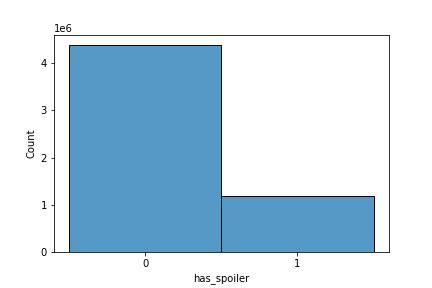
\includegraphics[width=\columnwidth]{img/imdb_classes.jpg}
    \caption{Class distribution in the IMDB dataset}
    \label{fig:imdb-classes}
\end{figure}

\begin{figure}[h]
    \centering
    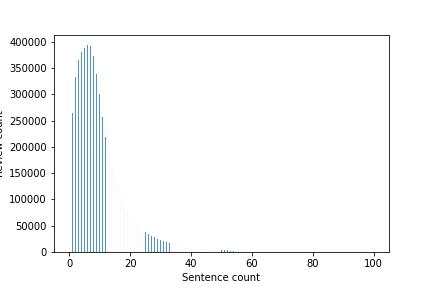
\includegraphics[width=\columnwidth]{img/imdb-sentence-length-hist.jpg}
    \caption{Histogram of review lengths w/o reviews with more than 100 sentences are not included}
    \label{fig:imdb-sentence-hist}
\end{figure}

\begin{table*}[t]
    \centering
    {\scriptsize
\begin{tabular}{|l|l|l|l|l|l|l|l|l|}
review\_id & reviewer        & movie                                                        & rating & review\_summary                                                                               & review\_date                                               & spoiler\_tag & review\_detail                                                                                & helpful                                                  \\\hline
rw0099142  & ed.wenn         & \begin{tabular}[c]{@{}l@{}}Le Samouraï\\ (1967)\end{tabular} & 9.0    & Cooler Than Cool                                                                              & \begin{tabular}[c]{@{}l@{}}26 November\\ 2000\end{tabular} & 0            & \begin{tabular}[c]{@{}l@{}}Surely one of the\\ suavest movies\\ ever made. Cr...\end{tabular} & \begin{tabular}[c]{@{}l@{}}{[}8,\\ 21{]}\end{tabular}    \\
rw0099143  & the red duchess & \begin{tabular}[c]{@{}l@{}}Le Samouraï\\ (1967)\end{tabular} & 10.0   & \begin{tabular}[c]{@{}l@{}}Along with\\ 'The Wizard of Oz',\\ the supreme fil...\end{tabular} & \begin{tabular}[c]{@{}l@{}}7 December\\ 2000\end{tabular}  & 1            & \begin{tabular}[c]{@{}l@{}}To see how\\ beautiful, moving,\\ exciting and ast...\end{tabular} & \begin{tabular}[c]{@{}l@{}}{[}219,\\ 284{]}\end{tabular}
\end{tabular}
}
    \caption{Sample of IMDB reviews dataset}
    \label{tab:imdb-sample}
\end{table*}



\section{Preliminary machine learning models}
In line with the approach proposed by Wróblewska \shortcite{wroblewska2021spoiler}, we have focused on state-of-the-art solutions based on transformer architecture. Namely, our current classifiers are built on BERT-based architectures. Apart from exploring the standard BERT Base-uncased model, we decided to try smaller DistilBERT architecture. Due to our computational limits, we felt it would be better to go this way rather than larger models such as the ELECTRA. According to the original paper, DistilBERT has 40\% fewer parameters than BERT Base-uncased and offers 60\% speedup. Table \ref{tab:bert-comparison} shows a more exact comparison.

\begin{table}[h]
    \centering
    \begin{tabular}{|c|c|}
        Model & \#Parameters \\\hline
        DistilBERT & 66M \\
        BERT & 110M
    \end{tabular}
    \caption{Comparison of used BERT-based base architectures}
    \label{tab:bert-comparison}
\end{table}



On top of the base architecture, we use a single fully-connected linear layer preceded by a dropout. Pooled BERT outputs serve as input for the dropout layer and final classification head.

Our initial experiments were conducted without the penultimate dropout layer, but we observed overfitting, so that's why we included it in further models. Additionally, we used pre-trained weights for BERT-based models. We were utilizing the Transformers library \cite{wolf-etal-2020-transformers}.

\section{Current experiments}

\subsection{Goodreads}

For the Goodreads dataset, we tested both DistilBERT as well as BERT models. 
The dataset was already split into train, test, and validation datasets. Each part was tokenized and converted to the TensorFlow Dataset class. It turned out that the training process took a long. Therefore, we have managed to train DistilBERT and BERT classifiers only for 3 epochs. The final dropout was set to 0.1. The initial learning rate was set to 2e-5 and followed by linear decay with Adam optimizer. Both models were trained using the balanced dataset and evaluated on both the balanced and entire datasets. The two datasets are disjoint, so we treat the former one as an enlarger train set.

Table \ref{tab:goodreads-results} contains results for DistillBERT and BERT. The lighter model with a significantly smaller number of parameters achieved only slightly worse results. The most notable difference occurs in the results for the entire imbalanced dataset, as shown in table \ref{tab:goodreads-results-full}. We will consider focusing solely on DistillBERT in the future to be able to conduct a larger number of experiments.  

\begin{table}[h]
    \centering
\begin{tabular}{|l|l|l|l|}
\begin{tabular}[c]{@{}l@{}}Classifier\\ architecture\end{tabular} & Accuracy & \begin{tabular}[c]{@{}l@{}}Balanced\\ accuracy\end{tabular} & ROC AUC \\ \hline
BERT                                                              & 0.8194   & 0.8199  & 0.9047 \\
\hline
DistilBERT                                                        & 0.8157   & 0.8162  & 0.8994
\end{tabular}
    \caption{Results achieved for the Goodread reviews test set}
    \label{tab:goodreads-results}
\end{table}


\begin{table}[h]
    \centering
\begin{tabular}{|l|l|l|}
\begin{tabular}[c]{@{}l@{}}Classifier\\ architecture\end{tabular} & Accuracy & ROC AUC \\ \hline
BERT                                                              & 0.8211   & 0.9022 \\
\hline
DistilBERT                                                        & 0.7778   & 0.8952
\end{tabular}
    \caption{Results achieved for the entire Goodreads reviews set}
    \label{tab:goodreads-results-full}
\end{table}

Note that in the presented experiments, all model weights were optimized. We also tried out freezing all pre-trained layers (except for the classification head), but it led to visibly worse results.


\subsection{TV Tropes Books}

Due to plans of combining the datasets to create a more general model, we decided on classifying the entire documents of TV Tropes as opposed to classifying individual sentences to either contain a spoiler or not. Such an approach slightly improves the balance of the dataset from 16\% of spoiler-tagged reviews to 22\%, which still makes a greatly imbalanced dataset. Not having access to a balanced version of it, we decided to account for the difference using class weights, which proved difficult due to the implementation of selected models and was ultimately postponed to a subsequent phase of the project. Augmentation of TV Tropes is another solution for the problem of imbalance to consider. Nevertheless, we conducted a training on TV Tropes Books without accounting for imbalance, using the same configuration as for the previous dataset. 

The results shown in table \ref{tab:tropes-results} exceeded our modest expectations and encouraged us to further investigate proposed improvements.

\begin{table}[]
    \centering
\begin{tabular}{|l|l|l|l|}
\begin{tabular}[c]{@{}l@{}}Classifier\\ architecture\end{tabular} & Accuracy & \begin{tabular}[c]{@{}l@{}}Balanced\\ accuracy\end{tabular} & ROC AUC \\ \hline
BERT                                                              & 0.8470   & 0.7418   & 0.8670                                                  
\end{tabular}
    \caption{Results achieved for the TV Tropes Books reviews test set}
    \label{tab:tropes-results}
\end{table}

\subsection{IMDB}
As mentioned before, we carried out experiments using a balanced IMDB dataset. It contained roughly 2.4M reviews, with half of it marked as spoilers. We split this balanced version into train, validation, and test parts in proportions of 0.8, 0.1, and 0.1.
Due to recurring training time issues, particularly pronounced in the case of IMDB, we used the same configuration of 3 epochs, final dropout set to 0.1, and Adam optimizer with decaying learning rate, starting from 2e-5. We saved the weights after the second epoch because the validation results were better compared to the end of the training.

Table \ref{tab:imdb-results} shows the results achieved on the test set. Here, we measured only the accuracy and balanced accuracy. Note that we didn't repeat the experiments, i.e., it was conducted only once. That's due to the learning time.

\begin{table}[h]
    \centering
\begin{tabular}{|l|l|l|}
\begin{tabular}[c]{@{}l@{}}Classifier\\ architecture\end{tabular} & Accuracy & \begin{tabular}[c]{@{}l@{}}Balanced\\ accuracy\end{tabular} \\ \hline
BERT                                                              & 0.7782   & 0.7783                                                     
\end{tabular}
    \caption{Results achieved for the IMDB reviews test set}
    \label{tab:imdb-results}
\end{table}

The results do not seem satisfactory. However, it was not our goal to build a powerful IMDB review classifier. Our aim is to utilize this task-related pre-trained model on other datasets, hoping for an improvement.




\section{Addressing weak points}
In the project proposal, we stated that the IMDB dataset, which we use, is rather rarely utilized in NLP works. We received a comment that this may not be true. We would therefore like to stress that the dataset we are using is different from a very popular IMDB reviews dataset introduced by Maas \shortcite{maas-EtAl:2011:ACL-HLT2011}. Note that the IMDB dataset which we explore contains about 5.5M reviews, while the second one features only 50K reviews. We agree that the latter dataset is widely known and often used for sentiment analysis, especially in some introductory materials. 

Still, we don't know whether a reviewer was aware of which specific dataset we decided to use. We do not deny that we may be wrong, and this large data set may often be used. We just want to make sure that the reader distinguishes between these two datasets.

In terms of risks regarding the datasets, we are optimistic, as the preliminary results show that while the training does, in fact, take a long time with prudently created experiments, it is manageable to use them.

Furthermore, we received a few comments about the presentation itself (both positive and negative). We will try our best to think through the presentation structure, manage our time, and provide illustrative examples to make the presentation more approachable and appealing.

Some weak points we couldn't understand, e.g., "Models are not transformers." During the presentation, we stated that we plan to use transformer-based models, and indeed they are transformer-based. Despite the fact whether the comment was on the basis of content or technicalities, we hope that the improvements to the presentation will resolve that.




\section{Summary}
In this document, we have shown our current progress. The next step is to incorporate XAI techniques into the developed models.


% include your bib file like this:
\bibliographystyle{acl}
\bibliography{bibliography}

\end{document}